\chapter{Flexion des mots composés}

\label{chap-multiflex}
MULTIFLEX est une plate-forme compatible Unicode de flexion automatique des \textit{mots composés}
ou \textit{multi-mots} (en anglais \textit{multi-word units}  MWUs).
\index{Multi-mots}\index{Mots composés}
Elle est tout particulièrement conçue pour la création de dictionnaires morphologiques de mots
composés.
Elle met en {\oe}uvre un formalisme fondé sur l'unification (\cite{Savary05}) 
pour la description du comportement flexionnel des mots composés et suppose l'existence d'un module
de flexion des mots simples.

\bigskip
\noindent Dans ce chapitre, nous présentons la notion de mots composés et nous décrivons la manière
de les fléchir avec MULTIFLEX.

\bigskip
\noindent Ce chapitre est fondé sur le manuel de MULTIFLEX, écrit par Agata Savary, l'auteur de
MULTIFLEX.

%%%%%%%%%%%%%%%%%%%%%%%%%%%%%%%%%%%%%%%%%%%%%%%%%%%%%%%%%%%%%
\section{Mots composés}
\label{section:MWUs}
Les mots composés (ou MWUs) englobent un ensemble d'objets linguistiques difficiles à définir et
contreversés  (cf. \cite{HabertJacquemin93}, \cite{Corbin92}). Leurs nombreuses définitions
linguistiques ou pragmatiques (\cite{Benven74}, \cite{Downing77}, \cite{Levi78}, 
\cite{Bauer83}, \cite{Gross90}, \cite{Anscombre90}, \cite{max-1993},
\cite{Gross96}, \cite{Cadiot92}) reposent sur trois principaux points:

\begin{itemize}
\item ils se composent de deux ou plusieurs mots
\item ils montrent un certain degré de non-compositionnalité sur le plan morphologique,
	distributionnel ou sémantique
\item ils possèdent un référent constant et unique
\end{itemize}

\bigskip
\noindent Cependant, les notions de base (un mot, un référent, la non-compositionnalité) et les
mesures (degré de non-compositionnalité) utilisées dans ces  définitions sont elles-mêmes
controversées.

\bigskip
\noindent De façon pragmatique, nous considérons comme mot composé une séquence d'\textit{unités
 graphiques} contiguës \index{Unité graphique} qui pour des raisons applicatives doivent être
 listées, décrites, (morphologiquement, syntaxiquement, sémantiquement, etc.) et traitées en tant
 qu'une seule et même unité.

 \subsection{Description formelle du comportement flexionnel des mots composés}
\label{subsec:MWUs inflection}
L'objectif principal de MULTIFLEX est le  mécanisme de flexion des mots composés.
Ce phénomène a été analysé en ce qui concerne l'anglais, le polonais et le français dans
\cite{these-Savary}.

\bigskip
\noindent Evidemment, un processus fiable de flexion des mots simples est un prérequis pour la
flexion des mots composés. Cependant, cette condition est rarement suffisante. Par exemple, en anglais, les
formes plurielles de 

\begin{itemize}
\item \emph{battle cry}
\item \emph{battle royal}
\item \emph{battle of nerves}
\end{itemize}

\noindent  il n'est pas seulement nécessaire de savoir comment générer les pluriels de 
\emph{battle, royal} et \emph{cry}, mais aussi de savoir quelles formes fléchies de ces constituants
se combinent entre elles:

\begin{itemize}
\item \emph{battle cr\underline{ies}}
\item \emph{battle royal\underline{s}}, or \emph{battle\underline{s} royal},
\item \emph{battle\underline{s} of nerves}
\end{itemize}

\noindent mais pas
 
\begin{itemize}
\item[*] {\emph{battle\underline{s} cr\underline{ies}}}
\item[*] {\emph{battle\underline{s} royal\underline{s}}}
\item[*] {\emph{battle\underline{s} of nerve\underline{ }}}
\end{itemize}

\bigskip
\noindent Formellement, une description explicite et complète du paradigme flexionnel des mots-composés doit répondre aux questions suivantes:

\begin{itemize}
\item A quelle catégorie grammaticale appartient le mot composé (nom, adjectif, etc.) et donc
quelles catégories flexionnelles (nombre, genre, cas, etc.) sont-elles pertinentes pour lui ?
\cite{PrzepWol03} se prononce pour une définiton fondée sur la morphosyntaxe des catégories
grammaticales : une catégorie grammaticale devrait pleinement déterminer les catégories
flexionnelles dans lesquelles le mot se fléchit ainsi que celles qui sont lexicalement fixées pour le
mot. Par exemple, en polonais, un nom a un genre et se fléchit en nombre et en cas.
\item Quelles sont les exceptions aux catégories flexionnelles déterminées ci-dessus ? Par exemple,
en polonais 

\begin{itemize}
\item \emph{wybory powszechne}\\
	(\emph{élections générales}) 
\end{itemize}

est un nom composé qui n'a pas de forme au singulier (cependant son nom tête \emph{wybory} en
	possède une).

\item Quelles sont les caractéristiques flexionnelles (forme canonique, catégorie grammaticale,
paradigme flexionnel, etc.) des constituants simples du mot composé ? Par exemple, en français,
\emph{porte} est un verbe non fléchi dans  

\begin{itemize}
\item \emph{porte-avion}
\end{itemize}

alors que c'est un nom fléchi dans
 
\begin{itemize}
\item \emph{porte-fenêtre}
\end{itemize}

qui prend un \emph{s} au pluriel

\begin{itemize}
\item \emph{porte\underline{s}-fenêtre\underline{s}}
\end{itemize}

\item Comment doit-on combiner les formes fléchies des constituants simples pour générer les formes fléchies du composé ? Par exemple, pour fléchir \emph{battle of nerves} et \emph{battle cry} nous devons fléchir respectivement le premier et le dernier constituant. 
\end{itemize}

%%%%%%%%%%%%%%%%%%%%%%%%%%%%%%%%%%%%%%%%%%%%%%%%%%%%%%%%%%%%%
\subsection{Approche lexicale ou grammaticale de la description morphologique}
Une étude précédente (\cite{these-Savary}) a confirmé le statut particulier des mots composés
les situant à la frontière de la morphologie et de la syntaxe. Leur structure compositionnelle
suggère une productivité qui ne pourrait guère être traitée sans une approche grammaticale. 

Toutefois, certaines de leurs propriétés morphologiques, syntaxiques et sémantiques excluent leur
traitement seulement en termes des propriétés de leurs constituants. Par exemple, dans les deux
exemples ci-dessous:

\begin{itemize}
\item \emph{chief justice}
\item \emph{lord justice}
\end{itemize} 

\noindent il y a peu d'indices automatiquement accessibles indiquant que le dernier est
morphologiquement un syntagme nominal anglais standard prenant un \emph{s} à son dernier constituant
au pluriel, tandis que le pluriel de celui-ci a trois variantes:
 
\begin{itemize}
\item \emph{chief justice\underline{s}}
\item \emph{lord justice\underline{s}, lord\underline{s} justice,
lord\underline{s} justice\underline{s}}
\end{itemize}
 
\bigskip
\noindent Ainsi, au moins l'un des exemples ci-dessus doit être considéré comme lexicalisé pour que
la flexion automatique soit fiable.

\bigskip
\noindent MULTIFLEX met en {\oe}uvre un formalisme fondé sur l'unification qui permet de décrire la
flexion des mots composés \cite{Savary05}. Ses caractéristiques sont décrites dans la
section~\ref{section:formalism}. Ce formalisme nécessite que la description soit \emph{pleinement}
lexicalisée: chaque mot composé figurant dans un dictionnaire est muni d'un code (ex: \emph{NC\_NN,
NC\_NN2}, etc.) représentant son paradigme flexionnel, par exemple, dans un format de type DELA:

\[
\begin{array}[c]{l}
  $aircraft carrier(carrier.N1:s),\textbf{NC\_NN}$ \\
  $chief justice(justice.N1:s),\textbf{NC\_NN}$ \\
  $lord(lord.N1:s) justice(justice.N1:s),\textbf{NC\_NN2}$ \\
  \dots
\end{array}
\]

\bigskip
\noindent Cependant, la grande majorité des mots composés peut être traitée avec un petit nombre de codes. Ainsi, la lexicalisation de la
description consiste principalement à définir les mots composés, qui respectent ou ne respectent pas
la  ``grammaire''.

%%%%%%%%%%%%%%%%%%%%%%%%%%%%%%%%%%%%%%%%%%%%%%%%%%%%%%%%%%%%%
\section{Formalisme de flexion des mots composés}
\label{section:formalism}
Un formalisme de description de la morphologie des mots composés a été décrit par Agata Savary en
1985 \cite{Savary05}. Il est fondé sur des études sur l'anglais, le polonais et le français, et
en outre a été testé pour le serbe \cite{Krstevetal06} et le grec \cite{Foufi13}.
Il repose sur une représentation indépendante de la langue qui doit être complétée par l'ensemble des éléments caractéristiques 
d'une langue donnée. Dans cette section, nous donnons une description détaillée de ce formalisme.

%%%%%%%%%%%%%%%%%%%%%%%%%%%%%%%%%%%%%%%%%%%%%%%%%%%%%%%%%%%%%
\subsection{Caractéristiques morphologiques de la langue}
\label{subsec:langfeat}
Lorsque l'on traite les mots composés d'une langue, il faut définir les caractéristiques générales
de cette langue. Ces données se trouvent dans deux fichiers textes.

\index{\verbc{Morphology.txt}}\index{Fichier!\verbc{Morphology.txt}}\bigskip
\noindent Le fichier \verb+Morphology.txt+  indique les catégories grammaticales
(nom, adjectif,\dots), catégories flexionnelles (nombre, genre, cas,\dots) et leurs valeurs 
(masculin, féminin, singulier, nominatif,\dots). Considérons l'exemple suivant:
\[
\begin{array}[c]{ll}
$Polish$ \\
$$<$CATEGORIES$>$$ \\
$Nb: sing, pl$ \\
$Case: Nom, Gen, Dat, Acc, Inst, Loc, Voc$ \\
$Gen: masc\_pers, masc\_anim, masc\_inanim, fem, neu$ \\
$$<$CLASSES$>$)$ \\
$noun: (Nb,$<$var$>$),(Case,$<$var$>$),(Gen,$<$fixed$>$)$ \\
$adj:(Nb,$<$var$>$),(Case,$<$var$>$),(Gen,$<$var$>$)$ \\
$adv:$
\end{array}
\]

\bigskip
\noindent Le fichier ci-dessus indique que pour le polonais, trois catégories flexionnelles sont
considérées: le nombre (\emph{Nb}), le cas (\emph{Case}), et le genre (\emph{Gen}). 
On donne pour chaque catégorie la liste exhaustive des valeurs qu'elle peut prendre (singulier et
pluriel pour le nombre, etc.).
Ensuite, chaque catégorie grammaticale est décrite selon les catégories qui varient avec la flexion,
et celles qui sont définies.
Par exemple, un nom se fléchit en nombre et en cas et possède un genre défini. 
Ce type de fichier est nécessaire pour exprimer le fait qu'un certain mot se fléchit en  nombre, genre ou cas, sans avoir à énumérer chaque fois les valeurs flexionnelles (singuler, pluriel, masculin, etc.) qu'il accepte.

\index{\verbc{Morphology.txt}}\index{Fichier!\verbc{Morphology.txt}}
\bigskip
\noindent De façon similaire, pour le français, le fichier \verb+Morphology.txt+ ressemble à ceci:
\[
\begin{array}[c]{l}
$French$ \\
$$<$CATEGORIES$>$$ \\
$Nb: s, p$ \\
$Gen: m, f$ \\
$$<$CLASSES$>$$\\
$noun: (Nb,$<$var$>$),(Gen,$<$var$>$)$ \\
$adj:(Nb,$<$var$>$),(Gen,$<$var$>$)$ \\
$adv:$
\end{array}
\]

\bigskip
\noindent Toutefois, dans les systèmes de flexion existants, de telles descriptions de catégories
grammaticales, catégories flexionnelles et valeurs ne sont pas toujours présentes. Par exemple,
selon les conventions DELA (\cite{dicos-francais}) les valeurs morphologiques des mots
simples sont des  séquences de  caractères contigus (e.g. \emph{ms} pour le  masculin singulier)
sans mention explicite des catégories correspondantes. Afin que le programme soit compatible avec de
tels systèmes, on utilise une liste (contenue dans le fichier appelé\index{\verbc{Equivalences.txt}}\index{Fichier!\verbc{Equivalences.txt}}
\verb+Equivalences.txt+) qui décrit quelle caractéristique flexionelle correspond à quelle paire
catégorie/valeur dans notre description. Par exemple, les listes suivantes:
\[
\begin{array}[c]{ll}
Polish                        &French\\
s: Nb=sing                    &s: Nb=s  \\
p: Nb=pl                      &p: Nb=p \\
M: Case=Nom                   &f: Gen=f  \\
D: Case=Gen                   &m: Gen=m    \\
C: Case=Dat  &\\
B: Case=Acc  &\\
I: Case=Inst  &\\
L: Case=Loc  &\\
V: Case=Voc  &\\
o: Gen=masc\_pers  &\\
z: Gen=masc\_anim  &\\
r: Gen=masc\_inanim  &\\
f: Gen=fem  &\\
n: Gen=neu &
\end{array}
\]

\bigskip
\noindent décrivent les équivalences entre les précédents fichiers \verb+Morphology.txt+
du polonais et du français, respectivement, et les caractéristiques représentées par une unique
lettre qui peuvent être utilisées dans les dictionnaires DELA pour ces langues dans Unitex.

%%%%%%%%%%%%%%%%%%%%%%%%%%%%%%%%%%%%%%%%%%%%%%%%%%%%%%%%%%%%%
\subsection{Décomposition d'un mot composé en constituants}
\label{subsec:decomp}
La notion de constituant élémentaire est controversée et varie selon les langues et les systèmes de
TAL. Par exemple, dans Unitex, un alphabet, c'est à dire un ensemble de caractères, est d'abord
défini pour chaque langue.  Tout caractère n'appartenant pas à l'alphabet est appelé séparateur. Un
constituant élémentaire est aussi bien un simple séparateur (habituellement un signe de ponctuation,
un chiffre, etc.) une séquence de caractères contigus appartenant à l'alphabet (ex
\emph{aujourd'hui} comporte selon cette définition, 3 constituants). Dans d'autres systèmes, un
constituant peut contenir un signe de ponctuation (e.g. \emph{c'est-\`a-dire}), ou une limite entre
deux constituants peut se produire dans une séquence de caractères alphabétiques (\emph{widzia\l
$\mid$bym} 'je verrais' , cf.
\cite{PrzepWol03}). 

\bigskip
\noindent Cette variété de définitions possibles d'un constituant a évidemment un impact sur la
définition d'un mot composé. Cependant, nous souhaitons que notre formalisme  puisse s'adapter à
différents systèmes de flexion de ``mots simples''. Ainsi, la définition d'un constituant est un
paramètre de notre système: chaque fois que MULTIFLEX est utilisé avec un module externe pour les
mots simples, celui-ci doit décider comment une séquence de caractères est divisée en constituants.

\bigskip
\noindent Dans notre formalisme, les constituants sont représentés par des variables numériques
\emph{\$1, \$2, \$3}, etc. 
Par exemple avec Unitex, la séquence

\begin{itemize}
\item \emph{Athens '04}
\end{itemize} 

\bigskip
\noindent comprend cinq constituants envoyés à MULTIFLEX de cette façon:
\[
\begin{array}[c]{l}
$\$1 = \emph{Athens}$ \\
$\$2 = $<$space$>$$ \\
$\$3 = \emph{'}$ \\
$\$4 = \emph{0}$ \\
$\$5 = \emph{4}$ \\
\end{array}
\]

\bigskip
\noindent Chaque constituant d'un mots composé suceptible d'être fléchi doit être morphologiquement 
identifié. Cette identification doit permettre de fournir les informations nécessaires afin que
n'importe quelle forme fléchie de ce mot puisse être générée à la demande. Par exemple dans:
\begin{itemize}
\item \emph{mémoire vive}
\end{itemize} 
nous devons savoir que \emph{vive} est le féminin singulier de \emph{vif}, et ainsi être capable de
générer le féminin pluriel, \emph{vives}. Dans MULTIFLEX nous supposons que ce module externe de
traitement des mots simples est responsable de leur identification et de la génération de leurs
formes fléchies.

\bigskip
\noindent Dans Unitex, la génération des formes fléchies est fortement inspirée du système DELA
(\cite{dicos-francais}). Pour générer une ou plusieurs formes fléchies d'un mot, nous devons
connaître:

\begin{itemize}
\item sa forme canonique
\item son paradigme flexionnel (appelé code flexionnel)
\item les caractéristiques flexionnelles des formes à produire
\end{itemize}

\bigskip
\noindent Ainsi, dans l'interface Unitex/MULTIFLEX la description d'un mot simple se fait comme suit
:

\begin{itemize}
\item \emph{vive(vif.A54:fs)}
\end{itemize} 

\bigskip
\noindent où \emph{A54} est le code flexionnel \emph{vif} et \emph{fs} forment la description
morphologique de type DELA des caractéristiques présentes dans le fichier \verb+Equivalences.txt+
(cf. section~\ref{subsec:langfeat}). En sachant que \emph{vive} est le féminin singulier de
\emph{vif}, on peut demander la génération du pluriel sans avoir à préciser explicitement le genre
du pluriel de la forme souhaitée: puisque nous voulons seulement modifier le nombre, le genre reste
celui du mot d'origine \emph{vive}, donc féminin.

\subsection{Paradigme de flexion des mots composés}
\label{subsec:paradigm}
Dans notre formalisme, la description morphologique des mots-composés repose sur le système DELA dans
la mesure où :

\begin{itemize}
\item chaque mot composé possède un code flexionnel
\item un code flexionnel décrit explicitement chaque forme fléchie en termes de traitement à
	effectuer sur sa forme canonique, et de caractéristiques à lui associer.
\end{itemize}

\bigskip
\noindent Dans sa version Unitex, MULTIFLEX utilise des codes flexionnels qui renvoient à des graphes
Unitex compilés au format\verb+.fst2+. Par exemple, figure~\ref{fig:BattleRoyal} présente le graphe de flexion pour \emph{battle royal}.

\begin{figure}[!htb]
  \centering
  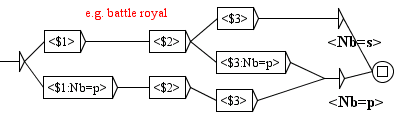
\includegraphics[width=10cm]{resources/img/BattleRoyal.png}
  \caption{Graphe de flexion pour \emph{battle royal}}
  \label{fig:BattleRoyal}
\end{figure}

\bigskip
\noindent Selon les conventions d'Unitex, trois constituants sont présents dans \emph{battle royal}:
\emph{battle} dénommé \emph{\$1}, un espace dénommé \emph{\$2}, et \emph{royal} dénommé \emph{\$3}.
Si des variables apparaissent seules dans une boîte, le constituant sera le même que dans le  lemme
du mot composé. Par exemple, $<$\$3$>$ dans le premier chemin du graphe signifie que \emph{royal}
doit être recopié tel quel. Si la variable est accompagnée d'assignations de la forme
catégories=caractéristiques, le constituant sera fléchi dans la forme demandée. Ainsi $<$\$3:Nb=p$>$
signifie que la  forme plurielle de \emph{royal} est souhaitée.

\bigskip
\noindent Pour générer toutes les formes fléchies d'un mot composé, nous devons explorer tous les
chemins du graphe. Chaque chemin débute à la flèche droite la plus à gauche et se termine à la 
boîte encerclée finale. Chaque fois qu'une boîte est atteinte, on réalise l'action qu'elle contient
(la recopie ou la flexion d'un constituant) et on accumule les informations présentes sous la boîte.
Le total des sorties des boîtes accumulé donne la description morphologique complète de la forme
fléchie.

\bigskip
\noindent Par exemple, dans le graphe de la figure~\ref{fig:BattleRoyal} si nous suivons le chemin
intermédiaire, extrait à la figure~\ref{fig:BattleRoyalonepath}:

\begin{figure}[!htb]
  \centering
  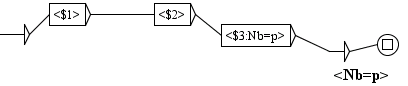
\includegraphics[width=10cm]{resources/img/BattleRoyalonepath.png}
  \caption{Un chemin du graphe de flexion de \emph{battle royal}}
  \label{fig:BattleRoyalonepath}
\end{figure}

\bigskip
\noindent nous recopions \emph{battle} (\emph{\$1}) et l'espace (\emph{\$2}), et nous mettons
\emph{royal} au pluriel, ce qui produit la forme du pluriel \emph{battle royals} du mot composé. Le
graphe de la figure~\ref{fig:BattleRoyal} contenant trois chemins différents, l'ensemble des formes
fléchies générées pour \emph{battle royal} sera: 
\[
\begin{array}[l]{l}
\emph{battle royal $<$Nb=s$>$} \\
\emph{battle royals $<$Nb=p$>$} \\
\emph{battles royal $<$Nb=p$>$}
\end{array}
\]
\bigskip
\noindent Après réécriture de ces formes au format DELACF, on obtient les entrées suivantes:
\[
\begin{array}[l]{l}
\emph{battle royal,battle royal.N:s} \\
\emph{battle royals,battle royal.N:p} \\
\emph{battles royal,battle royal.N:p}
\end{array}
\]

\bigskip
\noindent Remarquons que cette description est indépendante de la manière dont les formes fléchies
des mots simples sont générées parce que nous supposons que ce traitement est géré par le module
externe de flexion des mots simples. Dans la version Unitex de MULTIFLEX, nous générons le pluriel
de \emph{royal} du fait que nous connaissons son code flexionnel \emph{N1} qui correspond au graphe
de la figure \ref{fig:N1}.

\begin{figure}[!htb]
  \centering
  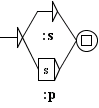
\includegraphics[width=2.8cm]{resources/img/N1'EN.png}
  \caption{Graphe de flexion \emph{N1} pour les mots simples qui se fléchissent comme \emph{royal}}
  \label{fig:N1}
\end{figure}

\bigskip
\noindent Dans le paradigme flexionnel d'un mot composé, chaque constituant est accompagné de la
catégorie morphologique qui détermine sa flexion. Les catégories inchangées n'ont pas besoin d'être
mentionnées. Par exemple, dans \emph{bateau-mouche} les deux noms constituants ont un genre
déterminé et ne se fléchissent qu'en nombre: \emph{bateau\underline{x}-mouche\underline{s}}. C'est
pourquoi (figure~\ref{fig:BateauMouche1}) dans le graphe de flexion de ce mot composé, les boîtes
correspondantes ne contiennent des assignations de  valeurs que pour le nombre. Remarquons que les
deux  constituants peuvent avoir ou non le même genre, ici \emph{bateau} est masculin tandis que
\emph{mouche} est féminin.

\begin{figure}[!htb]
  \centering
  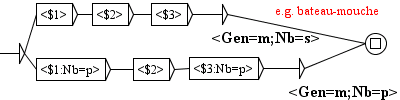
\includegraphics[width=10cm]{resources/img/BateauMouche1.png}
  \caption{Graphe de flexion pour les mots qui se fléchissent comme \emph{bateau-mouche}}
  \label{fig:BateauMouche1}
\end{figure}

%%%%%%%%%%%%%%%%%%%%%%%%%%%%%%%%%%%%%%%%%%%%%%%%%%%%%%%%%%%%%
\subsubsection{Variables d'unification}
Une caractéristique importante de notre formalisme est celle des \textit{variables d'unification}.
\index{Variable!d'unification}Elles sont représentées par un symbole dollar (\emph{\$}) suivi d'un identifiant pouvant
contenir n'importe quel nombre de caractères, comme \emph{\$g1}, \emph{\$num\_10}, \emph{\$c}, etc.
La figure~\ref{fig:BateauMouche2} montre un graphe approximativement équivalent\footnote{Même dans
le cas où les constituants simples apparaissant dans le lemme d'un mot composé sont déjà au
pluriel, comme dans \emph{cross-road\underline{s}}.} à celui de la figure~\ref{fig:BateauMouche1}
dans la mesure où il permet d'engendrer les mêmes formes fléchies pour le même mot composé.
Cependant, ici, un chemin unique représente à la fois le singulier et le pluriel. Ceci est rendu
possible grâce à la variable \emph{\$n} qui est instanciée tour à tour par toutes les valeurs du
domaine de sa catégorie (\emph{Nb}), ici \emph{\$n=s} puis \emph{\$n=p}.
Quand une variable d'unification apparait dans une formule du type \emph{Nb=\$n}, avec un seul signe égale
(=), le système parcourt toutes les valeurs déclarées dans les fichiers de configuration pour cette
catégorie (cf. section~\ref{subsec:langfeat}). Pour chaque valeur, il effectue une nouvelle instanciation
de la variable. L'instanciation est la même
pour tous les éléments du chemin: si une valeur est attribuée au premier constituant, la même valeur
doit être attribuée au troisième, ainsi que pour l'ensemble du mot composé. De même, si nous
attribuons à \emph{\$n} la valeur \emph{p} dans la première boîte, elle garde cette valeur \emph{p}
tout au long du chemin.

\begin{figure}[!htb]
  \centering
  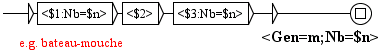
\includegraphics[width=10cm]{resources/img/BateauMouche2.png}
  \caption{Graphe de flexion avec variable pour les mots qui se fléchissent comme
  \emph{bateau-mouche}}
  \label{fig:BateauMouche2}
\end{figure}

\bigskip
\noindent Le graphe de flexion de la figure~\ref{fig:BateauMouche2} s'applique à la plupart des
composés français de types \emph{Nom Nom} et \emph{Nom Adjectif} (\emph{bateau-mouche, ange
gardien, circuit séquentiel}, etc.) qui sont de genre masculin~: c'est parce que la sortie de la 
boîte finale contient \emph{Gen=m}. Pour tous les composés des mêmes types, mais de genre féminin,
comme \emph{main courante, moissoneuse-batteuse}, etc., un nouveau graphe doit être créé, identique
à celui de figure~\ref{fig:BateauMouche2} jusqu'à la sortie finale contenant
\emph{$<$Gen=f;Nb=\$n$>$}.
Ce n'est pas très intuitif puisque \emph{circuit séquentiel} et \emph{main courante} se fléchissent
de la même manière, dans la mesure où dans les deux cas nous devons mettre au pluriel le premier et
le dernier constituant pour obtenir le pluriel du mot composé.

\bigskip
\noindent C'est pourquoi un autre type d'instanciation utilisant l'unification a été introduit. 
Il s'exprime au moyen de \emph{==} (par opposition au signe égale simple \emph{=} comme pour
\emph{\$n} dans la figure~\ref{fig:BateauMouche2}).
Quand une valeur est attribuée à une variable en utilisant ce symbole, la variable est instanciée une seule fois~:
elle hérite de la catégorie du
constituant, telle qu'elle apparaît dans la forme canonique du mot composé. Par exemple, la
figure~\ref{fig:BateauMouche3} contient un graphe décrivant la flexion pour le masculin comme pour
le féminin des mots composés de type \emph{Nom Nom} et \emph{Nom Adjectif}. La première boîte
contient l'affectation du genre par double signe égale pour la variable \emph{\$g}, ce qui signifie que cette
variable a pour genre celui du premier constituant. Pour \emph{bateau-mouche} c'est le masculin
parce que \emph{bateau} est masculin tandis que pour \emph{main courante} c'est le féminin. 

\begin{figure}[!htb]
  \centering
  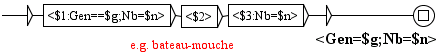
\includegraphics[width=11cm]{resources/img/BateauMouche3.png}
  \caption{Graphe de flexion \emph{bateau-mouche} avec deux types d'instanciation}
  \label{fig:BateauMouche3}
\end{figure}

\bigskip
\noindent Quand une affectation par double symbole égale coexiste avec une affectation par simple symbole égale,
sur le même chemin et pour la même variable, l'affectation par double symbole égale prévaut sur l'autre~: la
variable est instanciée une seule fois. Par exemple, sur la figure~\ref{fig:BateauMouche3} la sortie finale
contient \emph{Gen=\$g}, mais \emph{\$g} prend une seule valeur
déterminée par le premier constituant.

\bigskip
\noindent Le système d'unification est particulièrement utile pour des langues à la flexion riche.
Par exemple, en polonais la plupart des noms se fléchissent en nombre (2 valeurs) et en cas (7
valeurs), ce qui implique au moins 14 formes différentes (si des variantes et des formes
syncrétiques diffèrent).
Ce score est encore plus élevé pour les adjectifs qui se fléchissent en nombre, en cas et en genre
(de 3 à 9 valeurs, selon différentes approches). Si aucun mécanisme d'unification n'était
disponible, ces formes devraient être décrites par des chemins séparés dans le graphe.
L'unification permet de réduire considérablement la taille du graphe (jusqu'à un seul chemin dans la
plupart des cas).

\bigskip
\noindent Par exemple, le graphe de la figure~\ref{fig:PranieMozgu} permet de fléchir les mots
composés polonais qui se fléchissent comme \emph{pranie m\'ozgu} (\emph{lavage du cerveau}) ou
\emph{powo\.zenie koniem} (ang. \emph{horse coaching}). Leur troisième constituant a son cas défini
(le plus souvent au génitif ou à l'instrumental). Le premier et le troisième constituant se
fléchissent en nombre indépendamment l'un de l'autre  (\emph{pranie m\'ozg\underline{\'ow}},
\emph{prani\underline{a} m\'ozgu}, \emph{prani\underline{a} m\'ozg\underline{\'ow}}, etc.).
C'est pourquoi chacun d'eux a une variable différente pour la flexion en nombre  (\emph{\$n1} et
\emph{\$n2}). Les trois variables $\$n1$, $\$n2$, et $\$c$ peuvent être instanciées à n'importe
quelle valeur de leur domaine respectif  (\emph{\{sing,pl\}, \{sing,pl\}}, et
\emph{\{Nom,Gen,Dat,Acc,Inst,Loc,Voc\}}; cf. \verb+Morphology.txt+ fichier à la
section~\ref{subsec:langfeat}).
Le mot composé hérite son genre, son nombre et son cas de son premier constituant. Ce genre est
défini par (\emph{Gen==\$g}) alors que son nombre et son cas sont instanciés selon 14 combinaisons
possibles. Sans unification, le chemin unique de ce graphe aurait du être remplacé par 28 chemins
différents.

\begin{figure}[!htb]
  \centering
  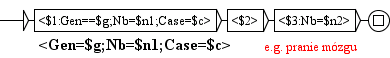
\includegraphics[width=10cm]{resources/img/PranieMozgu.png}
  \caption{Graphe de flexion pour \emph{pranie m\'ozgu}}
  \label{fig:PranieMozgu}
\end{figure}


%%%%%%%%%%%%%%%%%%%%%%%%%%%%%%%%%%%%%%%%%%%%%%%%%%%%%%%%%%%%%
\subsubsection{Variantes orthographiques et autres variantes}
Notre formalisme permet à n'importe quel constituant d'être omis ou déplacé au sein de différentes
formes fléchies si cela est nécessaire. Il permet également l'insertion de constituants
supplémentaires qui n'apparaissent pas dans la forme de base du mot composé. Cela permet d'étendre
un paradigme flexionnel à une description de variantes plus générale, orthographique ou, partielle,
variante syntaxique (voir \cite{Jacquemin01} pour une étude exhaustive des variantes).



Par exemple en anglais, 
\emph{student union} apparaît dans un corpus sous les formes \emph{student\underline{s} union}, et 
\emph{student\underline{s'} union}, au singulier ou au pluriel dans les deux cas. Notre formalisme 
permet d'ajouter les deux types de variantes à la description (cf. figure~\ref{fig:StudentUnion}).

\begin{figure}[!htb]
  \centering
  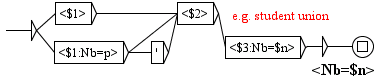
\includegraphics[width=10cm]{resources/img/StudentUnion.png}
  \caption{Graphe de flexion pour \emph{student union}}
  \label{fig:StudentUnion}
\end{figure}

\bigskip
\noindent figure~\ref{fig:BirthDate} montre un exemple dans lequel, en plus de l'insertion d'un
nouveau constituant, l'ordre des constituants peut être inversé. Le chemin du haut permet de
générer par exemple \emph{birth date} et \emph{birth dates} tandis que celui du bas représente
les variantes syntaxiques des formes précédentes: \emph{date of birth} et \emph{dates of birth}.

\begin{figure}[!htb]
  \centering
  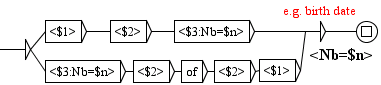
\includegraphics[width=10cm]{resources/img/BirthDate.png}
  \caption{Graphe de flexion pour \emph{birth date}}
  \label{fig:BirthDate}
\end{figure}

%%%%%%%%%%%%%%%%%%%%%%%%%%%%%%%%%%%%%%%%%%%%%%%%%%%%%%%%%%%%%
\subsubsection{Interface avec le système de flexion des mots simples}
\label{Interface}
MULTIFLEX est une mise en {\oe}uvre du formalisme de flexion des mots composés précédemment
présenté. Il suppose l'existence d'un sytème de flexion des mots simples qui satisfasse les
contraintes d'interface suivantes:

\begin{itemize}
\item Pour une séquence de caractères donnée, il renvoie sa décomposition en constituants insécables 
(tokens) (cf section~\ref{subsec:decomp}). Par exemple, dans le cas de la définiton d'un token dans
Unitex, la séquence \emph{Athens '04} est divisée en 5 tokens:
\[
\begin{array}[l]{l}
\emph{``Athens '04'' $\rightarrow$ (``Athens'','' ``,''''',''0'',''4'')}
\end{array}
\]

Pour une forme fléchie simple donnée, il retourne toutes ses caractéristiques flexionnelles. Ces
caractéristiques doivent permettre la génération à la demande de toute autre forme fléchie de même
lemme par le même module de flexion.
Par exemple, dans le cas d'Unitex, la forme \emph{porte} mène à  la reconnaissance de 7 formes 
(dont 6 sont factorisées selon leur code flexionnel):

\[
\begin{array}[l]{l}
\emph{porte $\rightarrow$ ((porte,porte.N21:s),(porte,porter.V3:P1s:P3s:S1s:S3s:Y2s))}
\end{array}
\]
En cas d'ambiguïté, comme ci-dessus, l'identification correcte doit être faite, pour le moment,
par l'utilisateur lors de l'édition du lemme du mot composé à fléchir (par la  suite, cette tâche
sera partiellement automatisée). Par exemple, dans le cas de \emph{porte-fenêtre}, le premier
constituant doit être identifié comme un nom plûtot que comme un verbe.

\item Pour une identification morphologique donnée et un ensemble de valeurs flexionnelles, il
renvoie toutes les formes fléchies corespondantes. Par exemple, en polonais, si le cas instrumental
du mot \emph{r\k{e}ka} doit être produit, trois formes doivent être renvoyées: \emph{r\k{e}k\k{a}} 
(instrumental singulier), \emph{r\k{e}kami} et  \emph{r\k{e}koma} (deux variantes de l'instrumental
pluriel).
\[
\begin{array}[l]{lll}
\emph{(r\k{e}ka,$<$Case=Inst$>$)}&  \rightarrow    &
\emph{((r\k{e}k\k{a},<Nb=sing;Gen=fem;Case=Inst>)}, \\
                                    &              & \emph{(r\k{e}kami,<Nb=pl;Gen=fem;Case=Inst>)},
                                    \\
                                    &              & \emph{(r\k{e}koma,<Nb=pl;Gen=fem;Case=Inst>))}
\end{array}
\]
\end{itemize}

\bigskip
\noindent La présence d'une interface entre le système de flexion des mots simples et celui des mots
composés permet une meilleure modularité et une indépendance de l'un vis-à-vis de l'autre. 
Le sytème de flexion des mots composés n'a pas besoin de savoir comment les formes fléchies des mots
simples sont décrites, analysées et générées. Il a seulement besoin d'un ensemble de formes
correctement fléchies des constituants des mots composés. Réciproquement, le système pour les mots
simples ne connait rien de la manière dont celui des mots composés combine les formes fournies.        
 
%%%%%%%%%%%%%%%%%%%%%%%%%%%%%%%%%%%%%%%%%%%%%%%%%%%%%%%%%%%%%
\section{Intégration à Unitex}
\label{section:UNITEXinterface}
L'un des principes majeurs de conception de MULTIFLEX est d'être aussi indépendant que possible du
système de flexion des mots simples. Cependant, l'existence d'un tel système est inévitable parce
qu'un mot composé est formé de mots simples que nous devons être en mesure de fléchir dans le but
de fléchir un mot composé dans son ensemble.

\bigskip
\noindent Dans sa version actuelle, MULTIFLEX repose sur le système de flexion des mots simples
d'Unitex

\begin{itemize}
\item MULTIFLEX utilise les mêmes codages qu'Unitex, i.e. Unicode 3.0.
\item MULTIFLEX utilise l'éditeur de graphe d'Unitex pour représenter la flexion des mots composés.
\item MULTIFLEX admet des principes de description morphologique similaires à ceux 
du système DELA mis en {\oe}uvre dans Unitex. Ainsi, un paradigme est un ensemble d'actions à effectuer sur le lemme afin de générer ses formes fléchies, et de leurs associer 
les informations flexionnelles correspondantes.
\item MULTIFLEX permet d'étendre la flexion des mots simples à celle des mots composés en produisant
à partir d'un DELAC (DELA électronique des mots composés) un DELACF (DELA électronique des formes
fléchies de mots composés).
Le format du DELACF généré est compatible avec Unitex tandis que le format du DELAC est nouveau,
mais inspiré de celui du DELAS (DELA électronique dictionnaire des mots simples).
\end{itemize}

\bigskip
\noindent Les sections suivantes présentent, pour plusieurs langues, des exemples complets de
flexion d'un DELAC en DELACF à travers l'interface MULTIFLEX/Unitex.

%%%%%%%%%%%%%%%%%%%%%%%%%%%%%%%%%%%%%%%%%%%%%%%%%%%%%%%%%%%%%
\subsection{Exemple complet en anglais}
Supposons que la description des caractéristiques morphologiques de l'anglais est définie par le
fichier \verb+Morphology.txt+ suivant:
\[
\begin{array}[l]{l}
$English$ \\
$<CATEGORIES>$ \\
$Nb:s,p$ \\
$<CLASSES>$ \\
$noun:(Nb,<var>)$ \\
$adj:$
\end{array}
\]

\bigskip
\noindent et que les équivalences entre les caractéristiques ci-dessus et leurs codes correspondants
dans les dictionnaires DELA sont définis par le fichier \verb+Equivalences.txt+ suivant: 
\[
\begin{array}[l]{l}
$English$ \\
$s : Nb=s$ \\
$p : Nb=p$ \\
\end{array}
\]

\bigskip
\noindent Considérons l'extrait du DELAC anglais suivant:

\begin{verbatim}
angle(angle.N1:s) of reflection,NC_NXXXX
Adam's apple(apple.N1:s),NC_XXXXN
air brake(brake.N1:s),NC_XXN
birth date(date.N1:s),NC_NN_NofN
criminal police,NC_XXXinv
cross-roads,NC_XXNs
head(head.N1:s) of government(government.N1:s),NC_NofNs
notary(notary.N3:s) public(public.N1:s),NC_NsNs
rolling stone(stone.N1:s),NC_XXN
student(student.N1:s) union(union.N1:s),NC_Ns'N
\end{verbatim}

\bigskip
\noindent Les graphes de flexion correspondants \emph{N1} et \emph{N3} pour les mots simples
se trouvent dans les figures~\ref{fig:N1'EN} et figures~\ref{fig:N3'EN} tandis que ceux pour les mots
composés s'échelonnent de la figure~\ref{fig:NC'NXXXX'EN} à la figure~\ref{fig:NC'Ns'N'EN}. 

\bigskip
\noindent Le DELACF résultant de la flexion par MULTIFLEX du DELAC précédent est le suivant:

\begin{verbatim}
angle of reflection,angle of reflection.NC_NXXXX:s
angles of reflection,angle of reflection.NC_NXXXX:p
Adam's apple,Adam's apple.NC_XXXXN:s
Adam's apples,Adam's apple.NC_XXXXN:p
air brake,air brake.NC_XXN:s
air brakes,air brake.NC_XXN:p
date of birth,birth date.NC_NN_NofN:s
dates of birth,birth date.NC_NN_NofN:p
birth date,birth date.NC_NN_NofN:s
birth dates,birth date.NC_NN_NofN:p
criminal police,criminal police.NC_XXXinv:p
cross-roads,cross-roads.NC_XXNs:s
cross-roads,cross-roads.NC_XXNs:p
heads of government,head of government.NC_NofNs:p
heads of governments,head of government.NC_NofNs:p
head of government,head of government.NC_NofNs:s
notaries public,notary public.NC_NsNs:p
notary public,notary public.NC_NsNs:s
notary publics,notary public.NC_NsNs:p
rolling stone,rolling stone.NC_XXN:s
rolling stones,rolling stone.NC_XXN:p
students' union,student union.NC_Ns'N:s
students' unions,student union.NC_Ns'N:p
students union,student union.NC_Ns'N:s
students unions,student union.NC_Ns'N:p
student union,student union.NC_Ns'N:s
student unions,student union.NC_Ns'N:p
\end{verbatim}
 
\begin{figure}[ht]
\begin{minipage}[c]{0.45\textwidth}
 \centering
 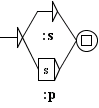
\includegraphics[width=2.5cm]{resources/img/N1'EN.png}
 \caption{Graphe de flexion \emph{N1} de mots simples anglais}
  \label{fig:N1'EN}
\end{minipage}\hfill
\begin{minipage}[c]{0.5\textwidth}
 \centering
 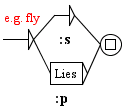
\includegraphics[width=3cm]{resources/img/N3'EN.png}
  \caption{Graphe de flexion \emph{N3} de mots simples anglais}
  \label{fig:N3'EN}
\end{minipage}
\end{figure}

%%%%%%%%%%%%MWUs

\begin{figure}[!htb]
  \centering
  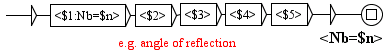
\includegraphics[width=10cm]{resources/img/NC'NXXXX'EN.png}
  \caption{Graphe de flexion \emph{NC\_NXXXX} de mots composés anglais}
  \label{fig:NC'NXXXX'EN}
\end{figure}

\begin{figure}[!htb]
  \centering
  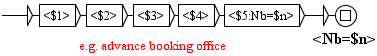
\includegraphics[width=9.7cm]{resources/img/NC'XXXXN'EN.png}
  \caption{Graphe de flexion \emph{NC\_XXXXN} de mots composés anglais}
  \label{fig:NC'XXXXN'EN}
\end{figure}

\begin{figure}[!htb]
  \centering
  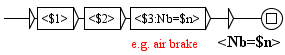
\includegraphics[width=7.8cm]{resources/img/NC'XXN'EN.png}
  \caption{Graphe de flexion \emph{NC\_XXN} de mots composés anglais}
  \label{fig:NC'XXN}
\end{figure}

\begin{figure}[!htb]
  \centering
  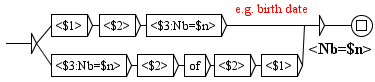
\includegraphics[width=10cm]{resources/img/NC'NN'NofN'EN.png}
  \caption{Graphe de flexion \emph{NC\_NN\_NofN} de mots composés anglais}
  \label{fig:NC'NN'NofN'EN}
\end{figure}

\begin{figure}[!htb]
  \centering
  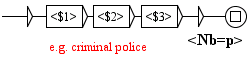
\includegraphics[width=7cm]{resources/img/NC'XXXinv'EN.png}
  \caption{Graphe de flexion \emph{NC\_XXXinv} de mots composés anglais}
  \label{fig:NC'XXXinv'EN}
\end{figure}

\begin{figure}[!htb]
  \centering
  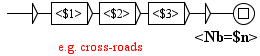
\includegraphics[width=7cm]{resources/img/NC'XXNs'EN.png}
  \caption{Graphe de flexion \emph{NC\_XXNs} de mots composés anglais}
  \label{fig:NC'XXNs'EN}
\end{figure}

\begin{figure}[!htb]
  \centering
  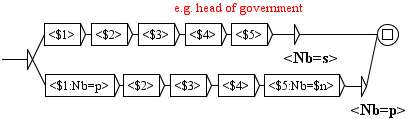
\includegraphics[width=10.4cm]{resources/img/NC'NofNs'EN.png}
  \caption{Graphe de flexion \emph{NC\_NofNs} de mots composés anglais}
  \label{fig:NC'NofNs'EN}
\end{figure}

\begin{figure}[!htb]
  \centering
  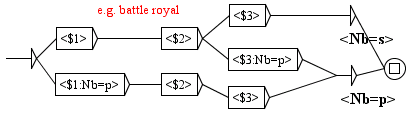
\includegraphics[width=10.4cm]{resources/img/NC'NsNs'EN.png}
  \caption{Graphe de flexion \emph{NC\_NsNs} de mots composés anglais}
  \label{fig:NC'NsNs'EN}
\end{figure}

\begin{figure}[!htb]
  \centering
  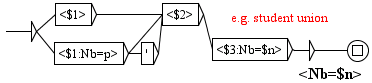
\includegraphics[width=9.8cm]{resources/img/NC'Ns'N'EN.png}
  \caption{Graphe de flexion \emph{NC\_Ns'N} de mots composés anglais}
  \label{fig:NC'Ns'N'EN}
\end{figure}

%%%%%%%%%%%%%%%%%%%%%%%%%%%%%%%%%%%%%%%%%%%%%%%%%%%%%%%%%%%%%
\subsection{Exemple complet en français}
Supposons que la description des caractéristiques morphologiques du français est définie par le
fichier \verb+Morphology.txt+ suivant:
\[
\begin{array}[l]{l}
$French$ \\
$<CATEGORIES>$ \\
$Nb : s, p$ \\
$Gen : m, f$ \\
$<CLASSES>$ \\
$noun : (Nb,<var>),(Gen,<var>)$ \\
$adj:(Nb,<var>),(Gen,<var>)$ \\
$adv:$
\end{array}
\]

\bigskip
\noindent et que les équivalences entre les caractéristiques ci-dessus et leurs codes correspondants
dans les dictionnaires DELA sont définis par le fichier \verb+Equivalences.txt+ suivant:

\[
\begin{array}[l]{l}
$French$ \\
$s : Nb=s$ \\
$p : Nb=p$ \\
$m : Gen=m$ \\
$f : Gen=f$
\end{array}
\]

\bigskip
\noindent Considérons l'extrait du DELAC français suivant (les codes flexionnels des mots simples
peuvent être différents de ceux présents dans Unitex):

\begin{verbatim}
avant-garde(garde.N21:fs),NC_XXN
bateau(bateau.N3:ms)-mouche(mouche.N21:fs),NC_NN
café(café.N1:ms) au lait,NC_NXXXX
carte(carte.N21:fs) postale(postal.A8:fs),NC_NN$
cousin(cousin.N8:ms) germain(germain.A8:ms),NC_NNmf
franc(franc.A47:ms) maçon(maçon.N41:ms),NC_AN1
mémoire(mémoire.N21:fs) vive(vif.A48:fs),NC_NN
microscope(microscope.N1:ms) à effet tunnel,NC_NXXXXXX
porte-serviette(serviette.N21:fs),NC_VNm
\end{verbatim}


\bigskip
\noindent Les graphes de flexion correspondants se trouvent de la figure ~\ref{fig:NC'XXN'FR} à la
figure ~\ref{fig:NC'VNm'FR}. 

\bigskip
\noindent Le DELACF résultant de la flexion par MULTIFLEX du DELAC précédent est le suivant:

\begin{verbatim}
avant-garde,avant-garde.NC_XXN:fs
avant-gardes,avant-garde.NC_XXN:fp
bateau-mouche,bateau-mouche.NC_NN:ms
bateaux-mouches,bateau-mouche.NC_NN:mp
café au lait,café au lait.NC_NXXXX:ms
cafés au lait,café au lait.NC_NXXXX:mp
carte postale,carte postale.NC_NN:fs
cartes postales,carte postale.NC_NN:fp
cousin germain,cousin germain.NC_NNmf:ms
cousins germains,cousin germain.NC_NNmf:mp
cousine germaine,cousin germain.NC_NNmf:fs
cousines germaines,cousin germain.NC_NNmf:fp
franc-maçon,franc maçon.NC_AN1:ms
franc-maçonne,franc maçon.NC_AN1:fs
franc maçon,franc maçon.NC_AN1:ms
franc maçonne,franc maçon.NC_AN1:fs
francs-maçons,franc maçon.NC_AN1:mp
francs-maçonnes,franc maçon.NC_AN1:fp
francs maçons,franc maçon.NC_AN1:mp
francs maçonnes,franc maçon.NC_AN1:fp
mémoire vive,mémoire vive.NC_NN:fs
mémoires vives,mémoire vive.NC_NN:fp
microscope à effet tunnel,microscope à effet tunnel.NC_NXXXXXX:ms
microscopes à effet tunnel,microscope à effet tunnel.NC_NXXXXXX:mp
porte-serviette,porte-serviette.NC_VNm:ms
porte-serviettes,porte-serviette.NC_VNm:ms
porte-serviettes,porte-serviette.NC_VNm:mp 
\end{verbatim}

\begin{figure}[!htb]
  \centering
  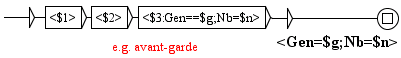
\includegraphics[width=10.2cm]{resources/img/NC'XXN'FR.png}
  \caption{Graphe de flexion \emph{NC\_XXN} de mots composés français}
  \label{fig:NC'XXN'FR}
\end{figure}

\begin{figure}[!htb]
  \centering
  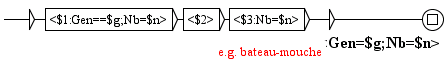
\includegraphics[width=10.8cm]{resources/img/NC'NN'FR.png}
  \caption{Graphe de flexion \emph{NC\_NN} de mots composés français}
  \label{fig:NC'NN'FR}
\end{figure}

\begin{figure}[!htb]
  \centering
  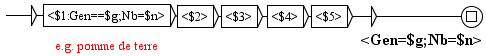
\includegraphics[width=12cm]{resources/img/NC'NXXXX'FR.png}
  \caption{Graphe de flexion \emph{NC\_NXXXX} de mots composés français}
  \label{fig:NC'NXXXX'FR}
\end{figure}

\begin{figure}[!htb]
  \centering
  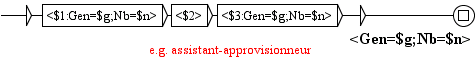
\includegraphics[width=12cm]{resources/img/NC'NNmf'FR.png}
  \caption{Graphe de flexion \emph{NC\_NNmf} de mots composés français}
  \label{fig:NC'NNmf'FR}
\end{figure}

\begin{figure}[!htb]
  \centering
  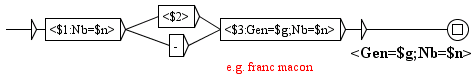
\includegraphics[width=12cm]{resources/img/NC'AN1'FR.png}
  \caption{Graphe de flexion \emph{NC\_AN1} de mots composés français}
  \label{fig:NC'AN1'FR}
\end{figure}

\begin{figure}[!htb]
  \centering
  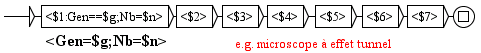
\includegraphics[width=12.2cm]{resources/img/NC'NXXXXXX'FR.png}
  \caption{Graphe de flexion \emph{NC\_NXXXXXX} de mots composés français}
  \label{fig:NC'NXXXXXX'FR}
\end{figure}

\begin{figure}[!htb]
  \centering
  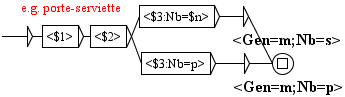
\includegraphics[width=9.2cm]{resources/img/NC'VNm'FR.png}
  \caption{Graphe de flexion \emph{NC\_VNm} de mots composés français}
  \label{fig:NC'VNm'FR}
\end{figure}


%\clearpage
\subsection{Exemple en serbe}
Supposons que la description des caractéristiques morphologiques du serbe est définie par le fichier
\verb+Morphology.txt+ suivant:
%\begin{comment}
\[
\begin{array}[l]{l}
$Serbian$\\
$<CATEGORIES>$\\
$Nb:s,p,w$ \\
$Case:1,2,3,4,5,6,7$\\
$Gen:m,f,n$\\
$Anim:v,q,g$\\
$Comp:a,b,c$\\
$Det:d,k,e$\\
$<CLASSES>$\\
$noun:(Nb,<var>),(Case,<var>),(Gen,<var>),(Anim,<fixed>)$\\
$adj:(Nb,<var>),(Case,<var>),(Gen,<var>),(Anim,<var>),(Comp,<var>),(Det,<var>)$\\
$adv:$
\end{array}
\]
%\end{comment}

\bigskip
\noindent La particuliarité de ce modèle morphologique n'est pas seulement sa richesse mais aussi
l'existence de \emph{no-care} features comme \emph{Anim=g} ou \emph{Det=e}. Ces caractéristiques 
s'accordent avec les autres caractéristiques de la même catégorie. Elles sont utilisées uniquement
pour certaines sous-classes particulières de noms ou d'adjectifs et sont nécessaires pour une
meill-eure compacité des paradigmes flexionnels des mots simples qui sont déjà très imposants, et le
seraient encore plus sans elles.

\bigskip
\noindent Supposons que les équivalences entre les caractéristiques ci-dessus et leurs codes
correspondants dans les dictionnaires DELA soient définis par le fichier \verb+Equivalences.txt+ suivant:

\[
\begin{array}[l]{l}
$Serbian$ \\
$s:Nb=s$ \\
$p:Nb=p$ \\
$w:Nb=w$ \\
$1:Case=1$ \\
$2:Case=2$ \\
$3:Case=3$ \\
$4:Case=4$ \\
$5:Case=5$ \\
$6:Case=6$ \\
$7:Case=7$ \\
$m:Gen=m$ \\
$f:Gen=f$ \\
$n:Gen=n$ \\
$v:Anim=v$ \\
$q:Anim=q$ \\
$g:Anim=g$ \\
$a:Comp=a$ \\
$b:Comp=b$ \\
$c:Comp=c$ \\
$d:Det=d$ \\
$k:Det=k$ \\
$e:Det=e$
\end{array}
\]

\bigskip
\noindent Considérons l'extrait du DELAC serbe suivant (les codes flexionnels des mots simples
peuvent être différents de ceux présents dans Unitex):
\scriptsize
\begin{verbatim}
zxiro racyun(racyun.N1:ms1q),NC_2XN1+N+Comp
avio-prevoznik(prevoznik.N10:ms1v),NC_2XN2+N+Comp
predsednik(predsednik.N10:ms1v) drzxave(drzxava.N600:fs2q),NC_N2X1+N+Comp
Ujedinxene(Ujedinxen.A1:aefp1g) nacije(nacija.N600:fp1q),NC_AXN3+N+Comp+NProp+Org
Kosovo(Kosovo.N308:ns1q) i Metohija(Metohija.N623:fs1q),NC_N3XN+N+Comp+NProp+Top+Reg 
istrazxni(istrazxni.A2:adms1g) sudija(sudija.N679:ms1v),NC_AXNF+N+Comp
Mirosinka(Mirosinka.N1637:fs1v) Dinkicx(Dinkicx.N1028:ms1v),NC_ImePrezime+N+Comp+Hum+PersName
gladan(gladan.A18:akms1g) kao vuk(vuk.N128:ms1v),AC_A3XN2/hungry as a wolf
\end{verbatim}
\normalsize

\bigskip
\noindent Les graphes de flexion correspondants se trouvent de la figure~\ref{fig:NC'2XN1'SRB} à la
figure~\ref{fig:AC'A3XN2'SRB}. 

\bigskip
\noindent Le DELACF résultant de la flexion par MULTIFLEX du DELAC précédent est le suivant:

\footnotesize
\begin{verbatim}
zxiro-racyun,zxiro racyun.NC_2XN1+N+Comp:s1qm
zxiro-racyuna,zxiro racyun.NC_2XN1+N+Comp:s2qm
zxiro-racyunu,zxiro racyun.NC_2XN1+N+Comp:s3qm
zxiro-racyun,zxiro racyun.NC_2XN1+N+Comp:s4qm
zxiro-racyune,zxiro racyun.NC_2XN1+N+Comp:s5qm
zxiro-racyunom,zxiro racyun.NC_2XN1+N+Comp:s6qm
zxiro-racyunu,zxiro racyun.NC_2XN1+N+Comp:s7qm
zxiro-racyuni,zxiro racyun.NC_2XN1+N+Comp:p1qm
zxiro-racyuna,zxiro racyun.NC_2XN1+N+Comp:p2qm
zxiro-racyunima,zxiro racyun.NC_2XN1+N+Comp:p3qm
zxiro-racyune,zxiro racyun.NC_2XN1+N+Comp:p4qm
zxiro-racyuni,zxiro racyun.NC_2XN1+N+Comp:p5qm
zxiro-racyunima,zxiro racyun.NC_2XN1+N+Comp:p6qm
zxiro-racyunima,zxiro racyun.NC_2XN1+N+Comp:p7qm
zxiro-racyuna,zxiro racyun.NC_2XN1+N+Comp:w2qm
zxiro-racyuna,zxiro racyun.NC_2XN1+N+Comp:w4qm
zxiro racyun,zxiro racyun.NC_2XN1+N+Comp:s1qm
zxiro racyuna,zxiro racyun.NC_2XN1+N+Comp:s2qm
zxiro racyunu,zxiro racyun.NC_2XN1+N+Comp:s3qm
zxiro racyun,zxiro racyun.NC_2XN1+N+Comp:s4qm
zxiro racyune,zxiro racyun.NC_2XN1+N+Comp:s5qm
zxiro racyunom,zxiro racyun.NC_2XN1+N+Comp:s6qm
zxiro racyunu,zxiro racyun.NC_2XN1+N+Comp:s7qm
zxiro racyuni,zxiro racyun.NC_2XN1+N+Comp:p1qm
zxiro racyuna,zxiro racyun.NC_2XN1+N+Comp:p2qm
zxiro racyunima,zxiro racyun.NC_2XN1+N+Comp:p3qm
zxiro racyune,zxiro racyun.NC_2XN1+N+Comp:p4qm
zxiro racyuni,zxiro racyun.NC_2XN1+N+Comp:p5qm
zxiro racyunima,zxiro racyun.NC_2XN1+N+Comp:p6qm
zxiro racyunima,zxiro racyun.NC_2XN1+N+Comp:p7qm
zxiro racyuna,zxiro racyun.NC_2XN1+N+Comp:w2qm
zxiro racyuna,zxiro racyun.NC_2XN1+N+Comp:w4qm
avio-prevoznik,avio-prevoznik.NC_2XN2+N+Comp:s1vm
avio-prevoznika,avio-prevoznik.NC_2XN2+N+Comp:s2vm
avio-prevozniku,avio-prevoznik.NC_2XN2+N+Comp:s3vm
avio-prevoznika,avio-prevoznik.NC_2XN2+N+Comp:s4vm
avio-prevoznicye,avio-prevoznik.NC_2XN2+N+Comp:s5vm
avio-prevoznikom,avio-prevoznik.NC_2XN2+N+Comp:s6vm
avio-prevozniku,avio-prevoznik.NC_2XN2+N+Comp:s7vm
avio-prevoznici,avio-prevoznik.NC_2XN2+N+Comp:p1vm
avio-prevoznika,avio-prevoznik.NC_2XN2+N+Comp:p2vm
avio-prevoznicima,avio-prevoznik.NC_2XN2+N+Comp:p3vm
avio-prevoznike,avio-prevoznik.NC_2XN2+N+Comp:p4vm
avio-prevoznici,avio-prevoznik.NC_2XN2+N+Comp:p5vm
avio-prevoznicima,avio-prevoznik.NC_2XN2+N+Comp:p6vm
avio-prevoznicima,avio-prevoznik.NC_2XN2+N+Comp:p7vm
avio-prevoznika,avio-prevoznik.NC_2XN2+N+Comp:w2vm
avio-prevoznika,avio-prevoznik.NC_2XN2+N+Comp:w4vm
avioprevoznik,avio-prevoznik.NC_2XN2+N+Comp:s1vm
avioprevoznika,avio-prevoznik.NC_2XN2+N+Comp:s2vm
avioprevozniku,avio-prevoznik.NC_2XN2+N+Comp:s3vm
avioprevoznika,avio-prevoznik.NC_2XN2+N+Comp:s4vm
avioprevoznicye,avio-prevoznik.NC_2XN2+N+Comp:s5vm
avioprevoznikom,avio-prevoznik.NC_2XN2+N+Comp:s6vm
avioprevozniku,avio-prevoznik.NC_2XN2+N+Comp:s7vm
avioprevoznici,avio-prevoznik.NC_2XN2+N+Comp:p1vm
avioprevoznika,avio-prevoznik.NC_2XN2+N+Comp:p2vm
avioprevoznicima,avio-prevoznik.NC_2XN2+N+Comp:p3vm
avioprevoznike,avio-prevoznik.NC_2XN2+N+Comp:p4vm
avioprevoznici,avio-prevoznik.NC_2XN2+N+Comp:p5vm
avioprevoznicima,avio-prevoznik.NC_2XN2+N+Comp:p6vm
avioprevoznicima,avio-prevoznik.NC_2XN2+N+Comp:p7vm
avioprevoznika,avio-prevoznik.NC_2XN2+N+Comp:w2vm
avioprevoznika,avio-prevoznik.NC_2XN2+N+Comp:w4vm
predsednik drzxave,predsednik drzxave.NC_N2X1+N+Comp:s1vm
predsednika drzxave,predsednik drzxave.NC_N2X1+N+Comp:s2vm
predsedniku drzxave,predsednik drzxave.NC_N2X1+N+Comp:s3vm
predsednika drzxave,predsednik drzxave.NC_N2X1+N+Comp:s4vm
predsednicye drzxave,predsednik drzxave.NC_N2X1+N+Comp:s5vm
predsednikom drzxave,predsednik drzxave.NC_N2X1+N+Comp:s6vm
predsedniku drzxave,predsednik drzxave.NC_N2X1+N+Comp:s7vm
predsednici drzxave,predsednik drzxave.NC_N2X1+N+Comp:p1vm
predsednici drzxava,predsednik drzxave.NC_N2X1+N+Comp:p1vm
predsednika drzxave,predsednik drzxave.NC_N2X1+N+Comp:p2vm
predsednika drzxava,predsednik drzxave.NC_N2X1+N+Comp:p2vm
predsednicima drzxave,predsednik drzxave.NC_N2X1+N+Comp:p3vm
predsednicima drzxava,predsednik drzxave.NC_N2X1+N+Comp:p3vm
predsednike drzxave,predsednik drzxave.NC_N2X1+N+Comp:p4vm
predsednike drzxava,predsednik drzxave.NC_N2X1+N+Comp:p4vm
predsednici drzxave,predsednik drzxave.NC_N2X1+N+Comp:p5vm
predsednici drzxava,predsednik drzxave.NC_N2X1+N+Comp:p5vm
predsednicima drzxave,predsednik drzxave.NC_N2X1+N+Comp:p6vm
predsednicima drzxava,predsednik drzxave.NC_N2X1+N+Comp:p6vm
predsednicima drzxave,predsednik drzxave.NC_N2X1+N+Comp:p7vm
predsednicima drzxava,predsednik drzxave.NC_N2X1+N+Comp:p7vm
predsednika drzxave,predsednik drzxave.NC_N2X1+N+Comp:w2vm
predsednika drzxava,predsednik drzxave.NC_N2X1+N+Comp:w2vm
predsednika drzxave,predsednik drzxave.NC_N2X1+N+Comp:w4vm
predsednika drzxava,predsednik drzxave.NC_N2X1+N+Comp:w4vm
Ujedinxene nacije,Ujedinxene nacije.NC_AXN3+N+Comp+NProp+Org:fp1q
Ujedinxenih nacija,Ujedinxene nacije.NC_AXN3+N+Comp+NProp+Org:fp2q
Ujedinxenima nacijama,Ujedinxene nacije.NC_AXN3+N+Comp+NProp+Org:fp3q
Ujedinxenim nacijama,Ujedinxene nacije.NC_AXN3+N+Comp+NProp+Org:fp3q
Ujedinxene nacije,Ujedinxene nacije.NC_AXN3+N+Comp+NProp+Org:fp4q
Ujedinxene nacije,Ujedinxene nacije.NC_AXN3+N+Comp+NProp+Org:fp5q
Ujedinxenima nacijama,Ujedinxene nacije.NC_AXN3+N+Comp+NProp+Org:fp6q
Ujedinxenim nacijama,Ujedinxene nacije.NC_AXN3+N+Comp+NProp+Org:fp6q
Ujedinxenima nacijama,Ujedinxene nacije.NC_AXN3+N+Comp+NProp+Org:fp7q
Ujedinxenim nacijama,Ujedinxene nacije.NC_AXN3+N+Comp+NProp+Org:fp7q
Kosovo i Metohija,Kosovo i Metohija.NC_N3XN+N+Comp+NProp+Top+Reg:ns1q
Kosova i Metohije,Kosovo i Metohija.NC_N3XN+N+Comp+NProp+Top+Reg:ns2q
Kosovu i Metohiji,Kosovo i Metohija.NC_N3XN+N+Comp+NProp+Top+Reg:ns3q
Kosovo i Metohiju,Kosovo i Metohija.NC_N3XN+N+Comp+NProp+Top+Reg:ns4q
Kosovo i Metohijo,Kosovo i Metohija.NC_N3XN+N+Comp+NProp+Top+Reg:ns5q
Kosovom i Metohijom,Kosovo i Metohija.NC_N3XN+N+Comp+NProp+Top+Reg:ns6q
Kosovu i Metohiji,Kosovo i Metohija.NC_N3XN+N+Comp+NProp+Top+Reg:ns7q
istrazxne sudije,istrazxni sudija.NC_AXNF+N+Comp:1vfp
istrazxnih sudija,istrazxni sudija.NC_AXNF+N+Comp:2vfp
istrazxnima sudijama,istrazxni sudija.NC_AXNF+N+Comp:3vfp
istrazxnim sudijama,istrazxni sudija.NC_AXNF+N+Comp:3vfp
istrazxne sudije,istrazxni sudija.NC_AXNF+N+Comp:4vfp
istrazxne sudije,istrazxni sudija.NC_AXNF+N+Comp:5vfp
istrazxnima sudijama,istrazxni sudija.NC_AXNF+N+Comp:6vfp
istrazxnim sudijama,istrazxni sudija.NC_AXNF+N+Comp:6vfp
istrazxnima sudijama,istrazxni sudija.NC_AXNF+N+Comp:7vfp
istrazxnim sudijama,istrazxni sudija.NC_AXNF+N+Comp:7vfp
istrazxne sudije,istrazxni sudija.NC_AXNF+N+Comp:2vfw
istrazxne sudije,istrazxni sudija.NC_AXNF+N+Comp:4vfw
istrazxnoga sudiju,istrazxni sudija.NC_AXNF+N+Comp:ms4v
istrazxnog sudiju,istrazxni sudija.NC_AXNF+N+Comp:ms4v
istrazxni sudija,istrazxni sudija.NC_AXNF+N+Comp:1vms
istrazxnoga sudije,istrazxni sudija.NC_AXNF+N+Comp:2vms
istrazxnog sudije,istrazxni sudija.NC_AXNF+N+Comp:2vms
istrazxnomu sudiji,istrazxni sudija.NC_AXNF+N+Comp:3vms
istrazxnome sudiji,istrazxni sudija.NC_AXNF+N+Comp:3vms
istrazxnom sudiji,istrazxni sudija.NC_AXNF+N+Comp:3vms
istrazxnomu sudiji,istrazxni sudija.NC_AXNF+N+Comp:7vms
istrazxnome sudiji,istrazxni sudija.NC_AXNF+N+Comp:7vms
istrazxnom sudiji,istrazxni sudija.NC_AXNF+N+Comp:7vms
istrazxni sudijo,istrazxni sudija.NC_AXNF+N+Comp:5vms
istrazxni sudija,istrazxni sudija.NC_AXNF+N+Comp:5vms
istrazxnim sudijom,istrazxni sudija.NC_AXNF+N+Comp:6vms
Dinkicx Mirosinka,Mirosinka Dinkicx.NC_ImePrezime+N+Comp+Hum+PersName:s1vf
Dinkicx Mirosinke,Mirosinka Dinkicx.NC_ImePrezime+N+Comp+Hum+PersName:s2vf
Dinkicx Mirosinki,Mirosinka Dinkicx.NC_ImePrezime+N+Comp+Hum+PersName:s3vf
Dinkicx Mirosinku,Mirosinka Dinkicx.NC_ImePrezime+N+Comp+Hum+PersName:s4vf
Dinkicx Mirosinka,Mirosinka Dinkicx.NC_ImePrezime+N+Comp+Hum+PersName:s5vf
Dinkicx Mirosinkom,Mirosinka Dinkicx.NC_ImePrezime+N+Comp+Hum+PersName:s6vf
Dinkicx Mirosinki,Mirosinka Dinkicx.NC_ImePrezime+N+Comp+Hum+PersName:s7vf
Mirosinka Dinkicx,Mirosinka Dinkicx.NC_ImePrezime+N+Comp+Hum+PersName:s1vf
Mirosinke Dinkicx,Mirosinka Dinkicx.NC_ImePrezime+N+Comp+Hum+PersName:s2vf
Mirosinki Dinkicx,Mirosinka Dinkicx.NC_ImePrezime+N+Comp+Hum+PersName:s3vf
Mirosinku Dinkicx,Mirosinka Dinkicx.NC_ImePrezime+N+Comp+Hum+PersName:s4vf
Mirosinka Dinkicx,Mirosinka Dinkicx.NC_ImePrezime+N+Comp+Hum+PersName:s5vf
Mirosinkom Dinkicx,Mirosinka Dinkicx.NC_ImePrezime+N+Comp+Hum+PersName:s6vf
Mirosinki Dinkicx,Mirosinka Dinkicx.NC_ImePrezime+N+Comp+Hum+PersName:s7vf
gladni kao vuk,gladan kao vuk.AC_A3XN2:s1mgda//hungry as a wolf
gladan kao vuk,gladan kao vuk.AC_A3XN2:s1mgka//hungry as a wolf
gladna kao vuk,gladan kao vuk.AC_A3XN2:s1fgea//hungry as a wolf
gladno kao vuk,gladan kao vuk.AC_A3XN2:s1ngea//hungry as a wolf
gladnoga kao vuk,gladan kao vuk.AC_A3XN2:s2mgda//hungry as a wolf
gladnog kao vuk,gladan kao vuk.AC_A3XN2:s2mgda//hungry as a wolf
gladna kao vuk,gladan kao vuk.AC_A3XN2:s2mgka//hungry as a wolf
gladne kao vuk,gladan kao vuk.AC_A3XN2:s2fgea//hungry as a wolf
gladnoga kao vuk,gladan kao vuk.AC_A3XN2:s2ngda//hungry as a wolf
gladnog kao vuk,gladan kao vuk.AC_A3XN2:s2ngda//hungry as a wolf
gladna kao vuk,gladan kao vuk.AC_A3XN2:s2ngka//hungry as a wolf
gladnome kao vuk,gladan kao vuk.AC_A3XN2:s3mgda//hungry as a wolf
gladnom kao vuk,gladan kao vuk.AC_A3XN2:s3mgda//hungry as a wolf
gladnu kao vuk,gladan kao vuk.AC_A3XN2:s3mgka//hungry as a wolf
gladnoj kao vuk,gladan kao vuk.AC_A3XN2:s3fgea//hungry as a wolf
gladnome kao vuk,gladan kao vuk.AC_A3XN2:s3ngda//hungry as a wolf
gladnom kao vuk,gladan kao vuk.AC_A3XN2:s3ngda//hungry as a wolf
gladnu kao vuk,gladan kao vuk.AC_A3XN2:s3ngka//hungry as a wolf
gladnu kao vuk,gladan kao vuk.AC_A3XN2:s4fgea//hungry as a wolf
gladno kao vuk,gladan kao vuk.AC_A3XN2:s4ngea//hungry as a wolf
gladni kao vuk,gladan kao vuk.AC_A3XN2:s5mgea//hungry as a wolf
gladna kao vuk,gladan kao vuk.AC_A3XN2:s5fgea//hungry as a wolf
gladno kao vuk,gladan kao vuk.AC_A3XN2:s5ngea//hungry as a wolf
gladnim kao vuk,gladan kao vuk.AC_A3XN2:s6mgea//hungry as a wolf
gladnom kao vuk,gladan kao vuk.AC_A3XN2:s6fgea//hungry as a wolf
gladnim kao vuk,gladan kao vuk.AC_A3XN2:s6ngea//hungry as a wolf
gladnome kao vuk,gladan kao vuk.AC_A3XN2:s7mgda//hungry as a wolf
gladnom kao vuk,gladan kao vuk.AC_A3XN2:s7mgda//hungry as a wolf
gladnu kao vuk,gladan kao vuk.AC_A3XN2:s7mgka//hungry as a wolf
gladnoj kao vuk,gladan kao vuk.AC_A3XN2:s7fgea//hungry as a wolf
gladnome kao vuk,gladan kao vuk.AC_A3XN2:s7ngda//hungry as a wolf
gladnom kao vuk,gladan kao vuk.AC_A3XN2:s7ngda//hungry as a wolf
gladnu kao vuk,gladan kao vuk.AC_A3XN2:s7ngka//hungry as a wolf
gladni kao vuk,gladan kao vuk.AC_A3XN2:p1mgea//hungry as a wolf
gladni kao vuci,gladan kao vuk.AC_A3XN2:p1mgea//hungry as a wolf
gladni kao vukovi,gladan kao vuk.AC_A3XN2:p1mgea//hungry as a wolf
gladne kao vuk,gladan kao vuk.AC_A3XN2:p1fgea//hungry as a wolf
gladne kao vuci,gladan kao vuk.AC_A3XN2:p1fgea//hungry as a wolf
gladne kao vukovi,gladan kao vuk.AC_A3XN2:p1fgea//hungry as a wolf
gladna kao vuk,gladan kao vuk.AC_A3XN2:p1ngea//hungry as a wolf
gladna kao vuci,gladan kao vuk.AC_A3XN2:p1ngea//hungry as a wolf
gladna kao vukovi,gladan kao vuk.AC_A3XN2:p1ngea//hungry as a wolf
gladnih kao vuk,gladan kao vuk.AC_A3XN2:p2mgea//hungry as a wolf
gladnih kao vuci,gladan kao vuk.AC_A3XN2:p2mgea//hungry as a wolf
gladnih kao vukovi,gladan kao vuk.AC_A3XN2:p2mgea//hungry as a wolf
gladnih kao vuk,gladan kao vuk.AC_A3XN2:p2fgea//hungry as a wolf
gladnih kao vuci,gladan kao vuk.AC_A3XN2:p2fgea//hungry as a wolf
gladnih kao vukovi,gladan kao vuk.AC_A3XN2:p2fgea//hungry as a wolf
gladnih kao vuk,gladan kao vuk.AC_A3XN2:p2ngea//hungry as a wolf
gladnih kao vuci,gladan kao vuk.AC_A3XN2:p2ngea//hungry as a wolf
gladnih kao vukovi,gladan kao vuk.AC_A3XN2:p2ngea//hungry as a wolf
gladnima kao vuk,gladan kao vuk.AC_A3XN2:p3mgea//hungry as a wolf
gladnima kao vuci,gladan kao vuk.AC_A3XN2:p3mgea//hungry as a wolf
gladnima kao vukovi,gladan kao vuk.AC_A3XN2:p3mgea//hungry as a wolf
gladnim kao vuk,gladan kao vuk.AC_A3XN2:p3mgea//hungry as a wolf
gladnim kao vuci,gladan kao vuk.AC_A3XN2:p3mgea//hungry as a wolf
gladnim kao vukovi,gladan kao vuk.AC_A3XN2:p3mgea//hungry as a wolf
gladnima kao vuk,gladan kao vuk.AC_A3XN2:p3fgea//hungry as a wolf
gladnima kao vuci,gladan kao vuk.AC_A3XN2:p3fgea//hungry as a wolf
gladnima kao vukovi,gladan kao vuk.AC_A3XN2:p3fgea//hungry as a wolf
gladnim kao vuk,gladan kao vuk.AC_A3XN2:p3fgea//hungry as a wolf
gladnim kao vuci,gladan kao vuk.AC_A3XN2:p3fgea//hungry as a wolf
gladnim kao vukovi,gladan kao vuk.AC_A3XN2:p3fgea//hungry as a wolf
gladnima kao vuk,gladan kao vuk.AC_A3XN2:p3ngea//hungry as a wolf 
gladnima kao vuci,gladan kao vuk.AC_A3XN2:p3ngea//hungry as a wolf
gladnima kao vukovi,gladan kao vuk.AC_A3XN2:p3ngea//hungry as a wolf
gladnim kao vuk,gladan kao vuk.AC_A3XN2:p3ngea//hungry as a wolf
gladnim kao vuci,gladan kao vuk.AC_A3XN2:p3ngea//hungry as a wolf
gladnim kao vukovi,gladan kao vuk.AC_A3XN2:p3ngea//hungry as a wolf
gladne kao vuk,gladan kao vuk.AC_A3XN2:p4mgea//hungry as a wolf
gladne kao vuci,gladan kao vuk.AC_A3XN2:p4mgea//hungry as a wolf
gladne kao vukovi,gladan kao vuk.AC_A3XN2:p4mgea//hungry as a wolf
gladne kao vuk,gladan kao vuk.AC_A3XN2:p4fgea//hungry as a wolf
gladne kao vuci,gladan kao vuk.AC_A3XN2:p4fgea//hungry as a wolf
gladne kao vukovi,gladan kao vuk.AC_A3XN2:p4fgea//hungry as a wolf
gladna kao vuk,gladan kao vuk.AC_A3XN2:p4ngea//hungry as a wolf
gladna kao vuci,gladan kao vuk.AC_A3XN2:p4ngea//hungry as a wolf
gladna kao vukovi,gladan kao vuk.AC_A3XN2:p4ngea//hungry as a wolf
gladni kao vuk,gladan kao vuk.AC_A3XN2:p5mgea//hungry as a wolf
gladni kao vuci,gladan kao vuk.AC_A3XN2:p5mgea//hungry as a wolf
gladni kao vukovi,gladan kao vuk.AC_A3XN2:p5mgea//hungry as a wolf
gladne kao vuk,gladan kao vuk.AC_A3XN2:p5fgea//hungry as a wolf
gladne kao vuci,gladan kao vuk.AC_A3XN2:p5fgea//hungry as a wolf
gladne kao vukovi,gladan kao vuk.AC_A3XN2:p5fgea//hungry as a wolf
gladna kao vuk,gladan kao vuk.AC_A3XN2:p5ngea//hungry as a wolf
gladna kao vuci,gladan kao vuk.AC_A3XN2:p5ngea//hungry as a wolf
gladna kao vukovi,gladan kao vuk.AC_A3XN2:p5ngea//hungry as a wolf
gladnima kao vuk,gladan kao vuk.AC_A3XN2:p6mgea//hungry as a wolf
gladnima kao vuci,gladan kao vuk.AC_A3XN2:p6mgea//hungry as a wolf
gladnima kao vukovi,gladan kao vuk.AC_A3XN2:p6mgea//hungry as a wolf
gladnim kao vuk,gladan kao vuk.AC_A3XN2:p6mgea//hungry as a wolf
gladnim kao vuci,gladan kao vuk.AC_A3XN2:p6mgea//hungry as a wolf
gladnim kao vukovi,gladan kao vuk.AC_A3XN2:p6mgea//hungry as a wolf
gladnima kao vuk,gladan kao vuk.AC_A3XN2:p6fgea//hungry as a wolf
gladnima kao vuci,gladan kao vuk.AC_A3XN2:p6fgea//hungry as a wolf
gladnima kao vukovi,gladan kao vuk.AC_A3XN2:p6fgea//hungry as a wolf
gladnim kao vuk,gladan kao vuk.AC_A3XN2:p6fgea//hungry as a wolf
gladnim kao vuci,gladan kao vuk.AC_A3XN2:p6fgea//hungry as a wolf
gladnim kao vukovi,gladan kao vuk.AC_A3XN2:p6fgea//hungry as a wolf
gladnima kao vuk,gladan kao vuk.AC_A3XN2:p6ngea//hungry as a wolf
gladnima kao vuci,gladan kao vuk.AC_A3XN2:p6ngea//hungry as a wolf
gladnima kao vukovi,gladan kao vuk.AC_A3XN2:p6ngea//hungry as a wolf
gladnim kao vuk,gladan kao vuk.AC_A3XN2:p6ngea//hungry as a wolf
gladnim kao vuci,gladan kao vuk.AC_A3XN2:p6ngea//hungry as a wolf
gladnim kao vukovi,gladan kao vuk.AC_A3XN2:p6ngea//hungry as a wolf
gladnima kao vuk,gladan kao vuk.AC_A3XN2:p7mgea//hungry as a wolf
gladnima kao vuci,gladan kao vuk.AC_A3XN2:p7mgea//hungry as a wolf
gladnima kao vukovi,gladan kao vuk.AC_A3XN2:p7mgea//hungry as a wolf
gladnim kao vuk,gladan kao vuk.AC_A3XN2:p7mgea//hungry as a wolf
gladnim kao vuci,gladan kao vuk.AC_A3XN2:p7mgea//hungry as a wolf
gladnim kao vukovi,gladan kao vuk.AC_A3XN2:p7mgea//hungry as a wolf
gladnima kao vuk,gladan kao vuk.AC_A3XN2:p7fgea//hungry as a wolf
gladnima kao vuci,gladan kao vuk.AC_A3XN2:p7fgea//hungry as a wolf
gladnima kao vukovi,gladan kao vuk.AC_A3XN2:p7fgea//hungry as a wolf
gladnim kao vuk,gladan kao vuk.AC_A3XN2:p7fgea//hungry as a wolf
gladnim kao vuci,gladan kao vuk.AC_A3XN2:p7fgea//hungry as a wolf
gladnim kao vukovi,gladan kao vuk.AC_A3XN2:p7fgea//hungry as a wolf
gladnima kao vuk,gladan kao vuk.AC_A3XN2:p7ngea//hungry as a wolf
gladnima kao vuci,gladan kao vuk.AC_A3XN2:p7ngea//hungry as a wolf
gladnima kao vukovi,gladan kao vuk.AC_A3XN2:p7ngea//hungry as a wolf
gladnim kao vuk,gladan kao vuk.AC_A3XN2:p7ngea//hungry as a wolf
gladnim kao vuci,gladan kao vuk.AC_A3XN2:p7ngea//hungry as a wolf
gladnim kao vukovi,gladan kao vuk.AC_A3XN2:p7ngea//hungry as a wolf
gladna kao vuk,gladan kao vuk.AC_A3XN2:w2mgea//hungry as a wolf
gladna kao vuci,gladan kao vuk.AC_A3XN2:w2mgea//hungry as a wolf
gladna kao vukovi,gladan kao vuk.AC_A3XN2:w2mgea//hungry as a wolf
gladne kao vuk,gladan kao vuk.AC_A3XN2:w2fgea//hungry as a wolf
gladne kao vuci,gladan kao vuk.AC_A3XN2:w2fgea//hungry as a wolf
gladne kao vukovi,gladan kao vuk.AC_A3XN2:w2fgea//hungry as a wolf
gladna kao vuk,gladan kao vuk.AC_A3XN2:w2ngea//hungry as a wolf
gladna kao vuci,gladan kao vuk.AC_A3XN2:w2ngea//hungry as a wolf
gladna kao vukovi,gladan kao vuk.AC_A3XN2:w2ngea//hungry as a wolf
gladna kao vuk,gladan kao vuk.AC_A3XN2:w4mgea//hungry as a wolf
gladna kao vuci,gladan kao vuk.AC_A3XN2:w4mgea//hungry as a wolf
gladna kao vukovi,gladan kao vuk.AC_A3XN2:w4mgea//hungry as a wolf
gladne kao vuk,gladan kao vuk.AC_A3XN2:w4fgea//hungry as a wolf
gladne kao vuci,gladan kao vuk.AC_A3XN2:w4fgea//hungry as a wolf
gladne kao vukovi,gladan kao vuk.AC_A3XN2:w4fgea//hungry as a wolf
gladna kao vuk,gladan kao vuk.AC_A3XN2:w4ngea//hungry as a wolf
gladna kao vuci,gladan kao vuk.AC_A3XN2:w4ngea//hungry as a wolf
gladna kao vukovi,gladan kao vuk.AC_A3XN2:w4ngea//hungry as a wolf
\end{verbatim}
\normalsize

\begin{figure}[!htb]
  \centering
  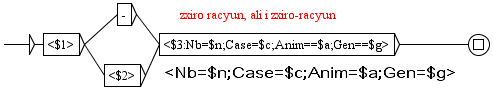
\includegraphics[width=12.4cm]{resources/img/NC'2XN1'SRB.png}
  \caption{Graphe de flexion \emph{NC\_2XN1} de mots composés serbes}
  \label{fig:NC'2XN1'SRB}
\end{figure}

\begin{figure}[!htb]
  \centering
  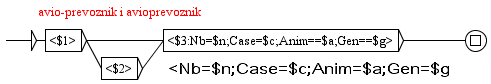
\includegraphics[width=12.4cm]{resources/img/NC'2XN2'SRB.png}
  \caption{Graphe de flexion \emph{NC\_2XN2} de mots composés serbes}
  \label{fig:NC'2XN2'SRB}
\end{figure}

\begin{figure}[!htb]
  \centering
  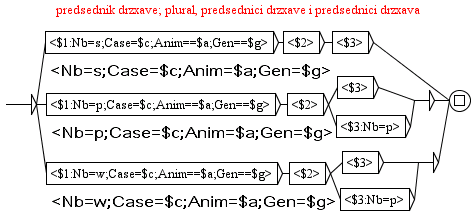
\includegraphics[width=12.2cm]{resources/img/NC'N2X1'SRB.png}
  \caption{Graphe de flexion \emph{NC\_N2X1} de mots composés serbes}
  \label{fig:NC'N2X1'SRB}
\end{figure}

\begin{figure}[!htb]
  \centering
  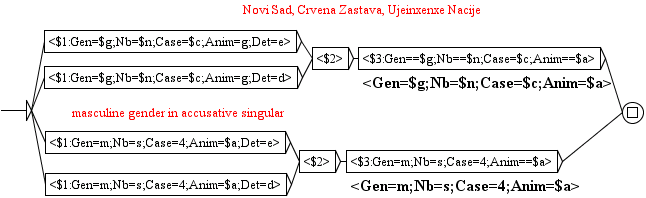
\includegraphics[width=15cm]{resources/img/NC'AXN3'SRB.png}
  \caption{Graphe de flexion \emph{NC\_AXN3} de mots composés serbes}
  \label{fig:NC'AXN3'SRB}
\end{figure}

\begin{figure}[!htb]
  \centering
  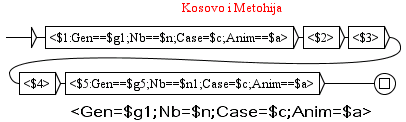
\includegraphics[width=10cm]{resources/img/NC'N3XN'SRB.png}
  \caption{Graphe de flexion \emph{NC\_N3XN} de mots composés serbes}
  \label{fig:NC'N3XN'SRB}
\end{figure}

\begin{figure}[!htb]
  \centering
  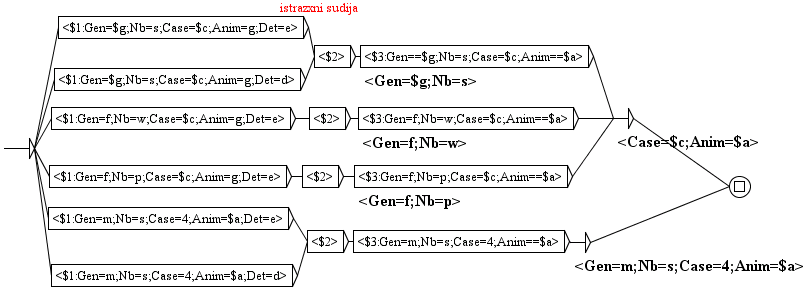
\includegraphics[width=15cm]{resources/img/NC'AXNF'SRB.png}
  \caption{Graphe de flexion \emph{NC\_AXNF} de mots composés serbes}
  \label{fig:NC'AXNF'SRB}
\end{figure}

\begin{figure}[!htb]
  \centering
  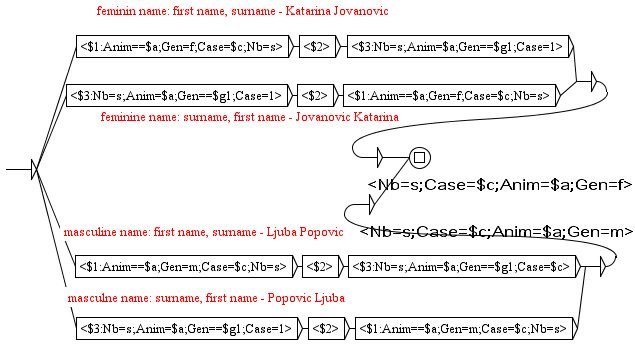
\includegraphics[width=15cm]{resources/img/NC'ImePrezime'SRB.png}
  \caption{Graphe de flexion \emph{NC\_ImePrezime} de mots composés serbes}
  \label{fig:NC'ImePrezime'SRB}
\end{figure}

\begin{figure}[!htb]
  \centering
  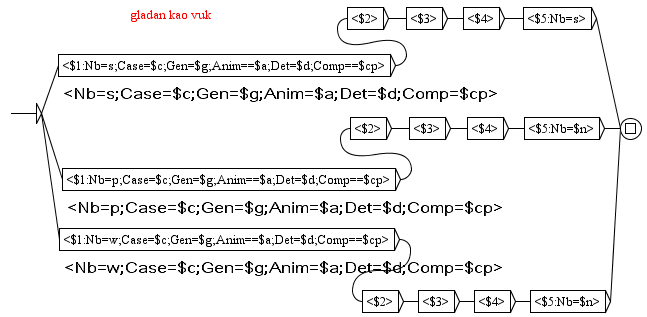
\includegraphics[width=15cm]{resources/img/AC'A3XN2'SRB.png}
  \caption{Graphe de flexion \emph{AC\_A3XN2} de mots composés serbes}
  \label{fig:AC'A3XN2'SRB}
\end{figure}

%%%%%%%%%%%%%%%%%%%%%%%%%%%%%%%%%%%%%%%%%%%%%%%%%%%%%%%
